\documentclass[we,twoside,openright,report,11pt]{uantwerpenthesistemplate}
%the first option is to define the colour scheme per faculty.
%Options are we (= sciences) or ti (= applied engineering)

%\documentclass{article}
%\usepackage{arxiv}
\usepackage[utf8]{inputenc}
\usepackage[T1]{fontenc}    % use 8-bit T1 fonts
\usepackage{hyperref}       % hyperlinks
 \usepackage{backref} % back references from the bibliography
\usepackage{url}            % simple URL typesetting
\usepackage{booktabs}       % professional-quality tables
\usepackage{amsfonts}       % blackboard math symbols
\usepackage{amsmath}
\usepackage{nicefrac}       % compact symbols for 1/2, etc.
\usepackage{microtype}      % microtypography
\usepackage{lipsum}
\usepackage{cite} % organizes citations
\usepackage{graphicx}
\usepackage{float}
\usepackage{subcaption}
\usepackage[ruled,vlined]{algorithm2e}
\usepackage{cleveref}
\usepackage{longtable}

%\usepackage[disable]{todonotes} %% Uncomment this line and comment the next one to make the notes invisible
\usepackage{todonotes}
\newcommand{\comment}[1]{\todo[color=orange!40, inline]{\footnotesize{#1}}}
\newcommand{\student}[1]{\todo[color=green!40, inline]{\footnotesize{Student: #1}}}
\newcommand{\serge}[1]{\todo[color=purple!40, inline]{\footnotesize{Serge: #1}}}



\hypersetup{
    colorlinks,%
    citecolor=black,%
    filecolor=black,%
    linkcolor=black,%
    urlcolor=black,
%
%    pdftitle={XXX},    % title
%    pdfauthor={XXX},     % author
%    pdfsubject={XXX},   % subject of the document
%    pdfcreator={PDF LaTex},   % creator of the document
}
\backrefsetup{verbose=false,hyperpageref}


\bamadegree{we-nl-ma-infse} %look up the encoding of this title in file uantwerpendocs-degree.data
% Options are 
%we-nl-ba-inf = Bachelor of Science in de informatica
%we-en-ma-infcn = Master of Science in computer science: computer networks
%we-en-ma-infdsai = Master of Science in computer science: data science and artificial intelligence
%we-en-ma-infse = Master of Science in computer science: software engineering
%we-nl-ma-infcn = Master of Science in de informatica: computernetwerken
%we-nl-ma-infdsai = Master of Science in de informatica: data science en artifici�le intelligentie
%we-nl-ma-infse = Master of Science in de informatica: software engineering

\title{Your Thesis Title}
\subtitle{Ommit subtitle if you don't have one}
\author{Student's Full Name}

\supervisor{prof. Prof. Serge Demeyer}{AnSyMo, UAntwerpen}
\cosupervisor{ing. P. Pienter}{AnSyMo, UAntwerpen}
\extsupervisor{dr. H. Warwinkel}{TNT-Bang, N.V.}

\academicyear{2022 - 2023}
\date{\today}


\begin{document}


\maketitle

\newpage
\tableofcontents
\newpage
\listoffigures
\newpage
\listoftables

\newpage
% !TEX root = ../Victorvan Herel2025_Thesis.tex

\setcounter{chapter}{-1}

\chapter{Preamble}

\section*{Abstract}
\addcontentsline{toc}{section}{Abstract}

Open source projects use software licensing as a tool to control how their software, and resulting forms such as compiled binaries, are used. However, people interacting with open source projects often do not have a background in law, and these software license texts are inherently legal in nature. This mismatch becomes relevant when project maintainers attempt to introduce code under a foreign license into their project, as the joined working of said license if often not immediately as easy to understand.

This thesis proposes a method to help alleviate this problem in a large number of cases, and draw attention to more cases which may cause problems. It does this by employing large language models to extract characteristics of licenses which can be easily understood by project maintainers, thus removing the need for a costly legal consultation.

\newpage
% !TEX root = ../Victorvan Herel2025_Thesis.tex

\section*{Nederlandstalige Samenvatting}
\addcontentsline{toc}{section}{Nederlandstalige Samenvatting}

Dutch Abstract.



\newpage
% !TEX root = ../Victorvan Herel2025_Thesis.tex

\section*{Acknowledgments}
\addcontentsline{toc}{section}{Acknowledgments}

Student's personal acknowledgements.

\newpage
% !TEX root = ../Victorvan Herel2025_Thesis.tex

\chapter{Introduction}\label{ch:introduction}

The introduction is probably the most important section of any academic work. 

A good way to structure an introduction is adopting the model of "Creating a Research Space" [C.A.R.S.] Model by John Swales. This model divides the typical intro into three "Moves".
\begin{itemize}
\item Move 1: Establishing a Territory [the situation]
\item Move 2: Establishing a Niche [the problem]
\item Move 3: Occupying the Niche [the solution]
\end{itemize}


We start the introduction with a small contextualization on the thesis/paper subject (i.e. "Move 1").
This usually takes 1 to 3 paragraphs for a paper depending on the topic. 
For a thesis, it is ok to write more paragraphs. 
Please remember, these are just general suggestions.

After the contextualization, we a few paragraph on the problem or motivation for this research  (i.e. "Move 2"). 
We should reinforce why the problem is important, why it is difficult, or how it affects academia and/or industry. 

After we successfully introduced the readers to the contextualization and problem/motivation, comes a paragraph clearly stating what is our research (i.e. "Move 3").
Usually, this paragraph begins with "In this paper/thesis, we ...".
Now the reader understands the basics of our research and what we did to accomplish our goals. 
The remaining paragraphs in the introduction can now describe a summary of the results, how previous research does not tackle what we did/accomplish, state the contributions for the research, or even an illustrative example of how the research improves the problem we described. 
The final paragraph of the introduction is an outline briefly describing the remaining sections. 
Use the \textbackslash ref\{...\} command to reference Sections and Chapters. 
For example, in Chapter~\ref{ch:background}, we describe...
And in Section~\ref{sec:ConceptA}, we describe...

\paragraph{LaTeX / Git tips and tricks}

Citations are very important in academic writing. 
Try to put at least one citation (preferable more) per paragraph in the introduction's previous paragraphs. 
Always use a citation when making a strong remark or statement to reinforce the point.
Example of citation~\cite{demeyer2002}.
For multiple citations put them all in the same cite command~\cite{vanbladel2020, parsai2020, njima2019, demeyer2002}. 
And yes, the tilde before the cite command is crucial -- it creates a small non-breaking space between the last word and the citation.
Remember that citations are annotations, not parts of speech.
Therefore do not use a citation as a substantive.

For Git-like repositories, try to put each sentence in a newline. 
Since Git is line-based, it makes it easier the see changes between versions.


\comment{We also included a comments command which makes it easier for students and advisors to give feedback or ask questions directly on the text. 
We can hide all comments in the pdf by changing a single line in the main tex file.}


\newpage
% !TEX root = ../Victorvan Herel2025_Thesis.tex

\chapter{Practical context}\label{ch:background}

Before we attempt to fomulate an answer to the questions proposed in Chapter~\ref{ch:introduction}, we first need to consider the context we are working in in a more concrete sense. This chapter examines existing standards and tools which are used by the industry to interact with software licenses, conflicts between them, compliance, ... right now.

\section{Accepted standards}\label{sec:context:standards}

To start, we would like to provide an overview of accepted standards in the industry which provide a leading effort in helping to handle complex software licensing interactions. These standards are listed in no particular order.

\begin{itemize}
	\item The \textbf{SPDX (System Package Data Exchange)} standard describes itself as "An open standard capable of representing systems with software components in as SBOMs (Software Bill of Materials) and other AI, data and security references supporting a range of risk management use cases.". To summarize, it is a way of including detailed licensing information right along with source code of the project in a standardized and well-defined way. This empowers projects such as ScanCode and FOSSology, which we will examine in the next section, to make very accurate reports of projects that employ the standard. It can also be employed for other use cases which are not relevant to this thesis, such as software security documentation.
	
	Aside from this, as a necessary addition, the SPDX standard also defines a set of licenses along with their license text which is immutable per published version of the standard. This is necessary as one of the standard's primary goals is facilitating software license compliance in a precise way. Having a fixed set of licenses to work with which each are provided with a fixed ID allows us to refer to licenses in very specific and unambiguous ways, provided they are part of the standard~\cite{spdx-home,spdx-licenses,spdx-explanation-1}.
	
	\item The \textbf{ReUse Software} project is an initiative by the Free Software Foundation Europe which provides a similar solution, profiling itself as an easy way to perform software license management in open source projects specifically. Like the SPDX standard, it provides tooling to add licensing information on a very granular level (up to individual files) within an open source code project. It improves the amount of projects automated scanning software can reliably analyse, with a focus on usability by project maintainers.
	
	This project does not provide a separate list of licenses, as it opts to make use of the SPDX license list~\cite{reuse-project-home}.
\end{itemize}

These standards are primarily practical ways with which individual project maintainers can improve legal legibility of their software code, and offer this thesis a stable source of license texts in the form of the SPDX license list, along with a way to refer to each license correctly in short. As an example, the MIT license simply has the identifier \verb*|MIT|. \\

\section{License scanners}\label{sec:license-scanners}

To perform license detection on projects that do not use either standard (though the listed scanners do fully support reading those), scanner software exists that generates reports on what licenses are in use in the project either directly or indirectly. The way these work differs, but the goal is the same, expanding the license horizon beyond what an individual project lists about itself.

\begin{itemize}
	\item The \textbf{ScanCode} project focuses on providing machine-readable compliance reports as well as human-readable reports on a software component's licensing information which includes that of its dependencies. It is able to analyse source code and binary files for these license and copyright statements and is actively used in the industry to visualize compliance information and improve discovery of problems related to it. It should be noted that it generally does not provide automated reasoning about license configurations outside of policies defined by its user~\cite{scancode-home}.
	
	\item Similarly the \textbf{FOSSology} project also offers the same scanning functionality, but focuses on workflow-based deployments rather than being able to be used ad-hoc and directly by project developers. It is targeted at actors within the industry for whom license compliance is a primary concern~\cite{fossology-home}.
	
	\item \textbf{Licensee} is a light-weight tool which does not provide a suite for gaining insight in how licenses are used in the project, including dependencies. Instead, its focus is correctly identifying license texts to an SPDX license ID in pre-determined locations. Usually the \verb*|LICENSE| file of a repository~\cite{licensee-scanner}.
	
	\item Other scanners do exist as well, but are usually part of enterprise-level all-in-one solutions. The license compliance part operates in generally the same way.
\end{itemize}

A key fact to consider is that while these scanners allow project maintainers to gain insight into their license usage, and even in some cases provide tooling to automatically check against certain policies the user defines, they do not provide any automated reasoning on their findings. If an incompatible license combination exists within a scanner's report, it is the responsibility of the user to flag it~\cite{scancode-home,fossology-home}. It is then a logical conclusion that the work presented in this thesis could be a first step to further improving the capabilities of these scanner projects.

\section{Custom licenses}\label{sec:custom-licenses}

While repository maintainers can choose to use a pre-defined license (often part of the SPDX license list), we recall that this action is, in a general sense, the person choosing the terms under which others can use their work. This does not have to be by choosing a pre-defined license, as one can instead decide to create their own.

While this is an option that is not often taken, as popular platforms such as GitHub encourage the use of a license upon creation of a repository to store code in~\cite{github_repository_creation}, custom licenses do exist and our thesis considers these as well. We show this fact by considering two avenues of reasoning:

\begin{itemize}
	\item The GitHub platform provides information on the number of repositories it hosts, and other metadata which can be consulted publicly. In this metadata, a project's primary license is listed as well. When one queries this data, an "Other" category is displayed which ranks third globally. This category contains all licenses which could not be identified by Licensee, the scanner which GitHub employs. This indicates that there is a very large number of repositories which use licenses that aren't known to the dataset it uses~\cite{github_innovation_graph_2025}.
	\item Widely used licenses were once defined by someone. As a result, within lists of publicly available licenses (SPDX, ScanCode, ...), we can often recognize names that refer to companies or industry actors. Licenses like the Pixar license, the radvd license, the PostgreSQL license, the Ruby License, ... are all examples of licenses that were made dedicated to a project, and may have gained traction and use in other projects since. This indicates that developers do indeed choose to make their own license if they cannot find an existing license that suits their need~\cite{spdx-licenses,scancode-licensedb}.
\end{itemize}

\section{License families}\label{sec:license-families}

While many different licenses exist, we can group them together into different license families based on their characteristics. This allows us to reason about groups of licenses in a general sense. The families of licenses relevant to this thesis are described here.

\subsection{Copyleft licenses}

A license that belongs in this family has a copyleft clause. This is a clause that requires that any derivative work created from the licensed work is also licensed under the same license, thus providing the work and any derivatives to the general public in an irrevocable way.

The point of copyleft licenses is to ensure the openness of the work by use of a license. Copyleft licenses require an author to make the work open source, and due to the reciprocity effect, any derivative works must also be made open source in turn under the same terms. This is a very strong requirement, and a sub-family which weakens this effect is the Copyleft Limited family, which does require source code redistribution for derivative works, but the obligation to redistribute source code of linked projects, some of which may be proprietary, is limited to provisions present in the license itself~\cite{scancode-licensedb,license-integration-patterns-1,license-integration-patterns-2}.

Well-known examples of the strong copyleft license family are the GPL and AGPL licenses. The Copyleft Limited license family is represented by the well known LGPL licenses~\cite{scancode-licensedb}.

\subsection{Permissive licenses}

The permissive licensing model creates an alternative approach to openness of the software. It does not impose the same limitation of which license derivative works must fall under. These licenses usually only require that the license text is retained along with the covered code in both source code and binary form, if those are provided to the general public and the covered code is contained within. This is as such a very open family of licenses, which places very reasonable conditions on usage of the work, but once satisfied, allows a wide range of permissions.

The permissive license family varies a lot, and as such there are no clear categories within it. These are not necessary however, as generally, two permissive licenses can work with each other, unless if provisions exist that conflict in both licenses~\cite{license-integration-patterns-1,license-integration-patterns-2}. It should be noted that in the next chapter, we will find that for within the ground truth of this thesis, no combination exists where two permissive licenses are incompatible with eachother.

\newpage
% !TEX root = ../Victorvan Herel2025_Thesis.tex

\chapter{Method}\label{ch:method}

\comment{!UNFINISHED CHAPTER! Here be dragons.}

For this thesis, we will be interfacing with large language models through the Ollama tool. We've selected this tool as we've found it to be very easy to use, providing a simple way to download models and subsequently querying them manually, or through an API which we can use in our reproduction package to automate certain tasks in obtaining our results~\cite{ollama_docs}.

For our methods proposed, we will perform this method on multiple LLM's to gauge their aptitude, and potentially also identify characteristics that an LLM should have to be able to give mostly correct answers. Where possible, we will aim for high decision accuracy on the question: Is a given combination of two licenses, where one is the leading license and the other the subordinate license, generally compatible? We do this to be able to dynamically construct a matrix in the same format of the license compatibility matrix provided by the OSADL.

\subsection{LLM selection}

For this thesis, we examine the LLM's outlined below. A general selection criterion was their availability. If an LLM is not openly available to run offline (with necessary preceeding downloads allowed), it is not the subject of this thesis as the goal is to provide a method that is open, and which anyone coming across the project could run on their own.

Aside from this criterion, we also clarify specific reasons for choosing a specific model as follows:
\begin{itemize}
	\item \textbf{Llama3:} A model which is indicated as being lightweight and general-purpose. This model does not feature a thinking property, which will generally make it faster than other models that do feature this property~\cite{ollama_llama3}. We include these non-thinking models in the proof-of-concept of this thesis to provide an indication of the trade-off between accuracy of prediction and prediction speed.
	\item \textbf{Gemma3:} This model is more recent compared to the Llama3 model, and as such it is a reasonable expectation for this model to perform better. Like Llama3, this model is a non-thinking model which is advertised to be capable of general-purpose language processing tasks~\cite{ollama_gemma3}.
	\item \textbf{Deepseek R1:} Deepseek R1 is the first model with a thinking property on this list. We also note that it is one of the first open models that feature this thinking capability~\cite{ollama_deepseekr1}. Generally, we expect this to be one of the better performing models because of its supposedly expanded reasoning capacity.
	\item \textbf{Qwen3:} The Qwen3 model is the most recently published model in the list of models this thesis uses. Like Deepseek R1, it features a thinking propert. It also advertises enhanced logical reasoning capacities, which are useful given the logical nature of the problems this thesis poses and seeks a solution to~\cite{ollama_qwen3}.
\end{itemize}

\subsection{Handling LLM stochasticity}

By design, large language models provide stochastic responses. This means that not every response generated by a model given an identical input will produce the same output, which provides a challenge to handle these responses automatically. How can we be certain that a model's answer is correct given the fact that it may answer differently given enough times to query the model identically? \\

This thesis will used a method inspired by ensemble classifiers in clustering problems to lessen the effect a stochasticly uncertain response may have on further reasoning based on it.

To do this, we will run each query-model combination multiple times, asking it questions which have a closed set of potential answers as much as possible. Where this isn't possible, such as with producing a list of license names, manual curation is needed to produce this closed answer set. For the example, this would be listing the SPDX license ID's for the license names produced. The final answer that will be regarded as the definitive answer of the model is the majority vote of the model's different responses over the answer sets. \\

A variable to consider is the amount of times a model is presented an identical query for this majority vote system. We will discuss the way this variable is determined inside the discussion of each of the methods, generally basing it on a border point where further querying is not likely to change a significant portion of the answers it provides on a question with a known ground truth. We will call this answer the \textbf{Majority-of-X} answer, where X is the number of queries used in determining said answer.

\section{PoC 1: Copyleft}

A first question this thesis aims to provide a proof of concept for is the ability for large language models to discern whether a given license text contains a copyleft clause. We do this as we recall that, in Chapter~\ref{ch:related-work}, we determined that the presence of a copyleft clause, and thus the license family to which a license belongs, is a strong indicator for determining further license configuration compatibilities.

\subsection{Approach}

With the models selected, we simply query the model for each license to obtain its answer to the question: Does this license text contain a copyleft clause?

This allows us to assign the license to a license family. We also have the ability to check this evaluation against a ground truth provided by the OSADL, which allows us to assess an accuracy score for each model across the entire dataset. It should be noted specifically, that we will \textbf{not} be considering the licenses of which the OSADL provides the answer: Questionable. We will still allow the models to assess these licenses, but for the purposes of calculating accuracy, we don't include these results as there is no ground-truth answer to compare to.\\

In order to address stochastic behavior which is inherent to large language models, we will query each model multiple times per query as indicated in the general notes section of this chapter.  \comment{Replace this with the border point of change\% approach.} This thesis has chosen to do this 5 times for each model, to weigh practicality of inference time with results.\\

The query each model is presented with for each run is the following, where the license's text is inserted in the indicated position:

\begin{verbatim}
	=== LICENSE FULL TEXT ===
	
	{license_fulltext}
	
	=== INSTRUCTION ===
	
	You are a license compatibility expert. Does the license contain a copyleft clause?
	A copyleft clause is a provision that requires derivative works to be distributed
	under the same license terms as the original work, ensuring that the freedoms
	granted by the license are preserved in derivative works.
	Begin your answer with a yes or a no for easy parsing.
\end{verbatim}

The license full text used is fetched from the SPDX license database, because of its comprehensive nature and ability to have fetching be fully automated based on SPDX license identifiers~\cite{spdx-licenses}. The SPDX license database is the most comprehensive authority of license texts which are meant for public use. Other tools such as ScanCode and FOSSology use SPDX license identifiers to refer to matched licenses~\cite{scancode-home}\cite{fossology-home}. \\

Lastly we remark that this query poses a yes/no question which limites the LLM to generating binary responses only. This is a required aspect of the \textbf{Majority-of-X} approach, as we need a closed answer set to determine a majority vote. For this proof of concept element, what is the majority is simply the majority vote on the single yes/no answers for a given query.

Lastly, we remark that a yes/no answer differs from the OSADL dataset described in Chapter~\ref{ch:related-work}, which also includes the does make a difference between strict and loosely copyleft. In the same chapter, we clarify that this generally does not make a difference and as such we don't need to further specify the answer. We also do not allow the LLM to produce the answer "Questionable", as to ensure it is able to provide an answer every time, rather than defaulting to the neutral answer for the more complex licenses.

\section{PoC 2: Explicit (in)compatibility}

\newpage
% !TEX root = ../Victorvan Herel2025_Thesis.tex

\chapter{Results}\label{ch:results}

\comment{!UNFINISHED CHAPTER! Here be dragons.}

\section{PoC 1: Copyleft clause detection results}

\subsection{Determining X for Majority-of-X}

As discussed in Chapter~\ref{ch:method}, we will first determine the value of X for a Majority-of-X answer construction. To do this, we need a border point \comment{Victor: Fill this with requirements for a border point.}. \\

After running the models for multiple times, we can render the following table of the first 15 Majority-of-X answers. It is important to understand that order is always preserved in these answers.

\begin{tabular}{|l|ccccccccccccccc|}
	\hline& \multicolumn{15}{|c|}{\textbf{Majority-of-X accuracy (all licenses in dataset with known truth)}} \\
	\multicolumn{1}{|r|}{\textbf{X = $\ldots$}} & \textbf{1} & \textbf{2} & \textbf{3} & \textbf{4} & \textbf{5} & \textbf{6} & \textbf{7} & \textbf{8} & \textbf{9} & \textbf{10} & \textbf{11} & \textbf{12} & \textbf{13} & \textbf{14} & \textbf{15} \\\hline
	Llama3 & 001 & 002 & 003 & 004 & 005 & 006 & 007 & 008 & 009 & 010 & 011 & 012 & 013 & 014 & 015 \\
	Gemma3 & 1 & 2 & 3 & 4 & 5 & 6 & 7 & 8 & 9 & 10 & 11 & 12 & 13 & 14 & 15 \\
	Deepseek R1 & 1 & 2 & 3 & 4 & 5 & 6 & 7 & 8 & 9 & 10 & 11 & 12 & 13 & 14 & 15 \\
	Qwen3 & 1 & 2 & 3 & 4 & 5 & 6 & 7 & 8 & 9 & 10 & 11 & 12 & 13 & 14 & 15 \\\hline
\end{tabular}

\subsection{Accuracy scoring}

We consider the results of the copyleft detection experiment first as follows: \\

\textbf{Llama3:8n:} Upon a first run of this model with the given task, it was decided not to continue with the additional runs for this model, as its accuracy was already very low and as such Llama3:8b is not a promising avenue compared to other selected models. The confusion matrix for this run is provided in Table~\ref{tab:llama3-1-confmatrix}. This run scores an accuracy of \textbf{55.17\% (64 / 116)}. While the mistakes made by this model are varied, it is clear the model particularly struggles with false positive detections of a copyleft clause.

\begin{table}[h]
	\caption{Llama3:8b confusion matrix (Run 1/1)}
	\label{tab:llama3-1-confmatrix}
	\centering
	\begin{tabular}{l|ll}
		\hline
		\textbf{LLM \textbackslash OSADL} & Copyleft & Permissive \\ \hline
		Copyleft & 25 & 48 \\
		Permissive & 4 & 39 \\\hline
	\end{tabular}
\end{table}

\textbf{Gemma3:4b:} This model performed better, scoring an average accuracy across runs of 83.62\% (97/116). Its mistakes are also exclusively failures to detect a present copyleft license. The confusion matrix for the majority vote is given in Table~\ref{tab:gemma3-confmatrix}, which scored the same accuracy as the average accuracy. The model is very consistent, only differing in responses across runs for the MPL-1.1 license and the MPL-2.0-no-copyleft-exception license.

\textbf{Average accuracy:} 83.62\% (97 / 116)

\textbf{Majority-of-5 accuracy:} 83.62\% (97 / 116)

\begin{table}[h]
	\caption{Gemma3:4b confusion matrix (Majority vote of 5 runs)}
	\label{tab:gemma3-confmatrix}
	\centering
	\begin{tabular}{l|ll}
		\hline
		\textbf{LLM \textbackslash OSADL} & Copyleft & Permissive \\ \hline
		Copyleft & 10 & 0 \\
		Permissive & 19 & 87 \\\hline
	\end{tabular}
\end{table}

\textbf{Deepseek R1:8b:} This model is very inconsistent with its answers, answering differently across runs for 28 licenses in the dataset. Additionally, this model classifies 2 specific licenses incorrectly on all its runs. We will discuss this rather peculiar result after the listing of direct results. In a majority configuration however, we note that the accuracy increases (107 licenses correctly classified, as opposed to 104 in the best run). This suggests that this model does benefit from a majority vote setup. Notably, this model also does not make any false positive detections.

\textbf{Average accuracy:} 88.62\% (\~ 102.8 / 116)

\textbf{Majority-of-5 accuracy:} 92.24\% (107 / 116)

\begin{table}[h]
	\caption{Deepseek R1:8b confusion matrix (Majority vote of 5 runs)}
	\label{tab:deepseekr1-confmatrix}
	\centering
	\begin{tabular}{l|ll}
		\hline
		\textbf{LLM \textbackslash OSADL} & Copyleft & Permissive \\ \hline
		Copyleft & 20 & 0 \\
		Permissive & 9 & 87 \\\hline
	\end{tabular}
\end{table}

- Qwen3:8b: This model is the best model of the selected models for this task. It however doesn't really benefit from the majority vote decision setup, like we have seen for the Deepseek model. Instead, its runs generally are very accurate, outclassing all other 3 models that were included in this experiment, however the best run actually performs better than the majority vote, correctly classifying 113 out of 116 licenses. We see in the confusion matrix that this model does make false positive classifications, as opposed to the other two models which do not make this mistake.

\textbf{Average accuracy:} 96.21\% (\~ 111.6 / 116)

\textbf{Majority-of-5 accuracy:} 96.55\% (112 / 116)

\begin{table}[h]
	\caption{Qwen3:8b confusion matrix (Majority vote of 5 runs)}
	\label{tab:qwen3-confmatrix}
	\centering
	\begin{tabular}{l|ll}
		\hline
		\textbf{LLM \textbackslash OSADL} & Copyleft & Permissive \\ \hline
		Copyleft & 26 & 1 \\
		Permissive & 3 & 86 \\\hline
	\end{tabular}
\end{table}

\section{Examining mistakes made by models}

\subsection{General mistakes}

The Gemma3, Deepseek R1 and Qwen3 model all failed to classify two licenses correctly, looking into the thinking of the models when making this decision, we can explain why:
\begin{itemize}
	\item \textbf{IPL-1.0:} The IBM Public License is a complex case because it handles source code redistribution and binary object redistribution entirely differently. We examine specifically its Section 3 Requirements. This mentions the following:
	\begin{itemize}
		\item "When the Program is made available in source code form: a. it must be made available under this Agreement; and b. a copy of this Agreement must be included with each copy of the Program." This section tells us that source code redistribution is strongly copyleft, requiring the same license is used for the derivative work created.
		\item "A contributor may choose to distribute the Program in object code form under its own license agreement, provided that: [...]" This section governs binary delivery, and it does impose that whichever license agreement you use, it complies with the IPL-1.0, and must disclaim warranty on behalf of the contributors, excluding them from liabilities, damages, ... much like the MIT license. It goes on to permit the new license to differ, but that such different clauses are only offered by the redistributing contributor alone.
		This difference between handling of source code redistribution and binary object redistribution seems to confuse our models. The option to redistribute under a different license, given specific requirements, is not a copyleft clause. As such, the models decide to classify this license as permissive in all runs.
	\end{itemize}
	
	\item \textbf{Sleepycat:} The sleepycat license is also always classified incorrectly. In this case, the source of confusion is very obvious. The sleepycat license itself is actually 3 licenses which were concatenated together. Because of this, and the predictable nature of the format of these licenses, the models get confused when running inference, treating each license referenced as a separate question. As a result, it fails to comply with the answer format provided, meaning automatic detection of the answer fails as well for Deepseek R1 and Qwen3. For Gemma3, it actually is capable of considering the entire license as its own block, however it is mistaken in handling of the license itself, missing the fact that the Sleepycat section of this license is indeed BSD-3 Clause, but adds an additional clause which imposes a Copyleft clause to this format.
\end{itemize}

\subsection{Individual mistakes}

An interesting mistake only made by the Qwen3 model occurs when examining the Artistic-2.0 license. Gemma3 and Deepseek R1 remain faultless here. This mistake seems to stem from Clause 4a in the license, which \textit{is} a copyleft license, but is preceeded by a construct that indicates this is optional if compliance is instead ensured with clause 4b or clause 4c in the license, which are not copyleft clauses. In a sense, Qwen3 correctly answers the question posed, as this simply queries the model for a Yes/No answer to the question: "Does this license contain a copyleft clause?". This differs from being a part of the copyleft license family.

Other mistakes do not appear to form a coherent pattern. Additionally, among the list of most used licenses according to GitHub's Innovation Graph project, mistakes still get made by Gemma3 and Deepseek R1 within this subset. Qwen3 remains faultless within this subset across all of the recorded runs~\cite{github_innovation_graph_2025}.

This list of frequently used licenses is included in this document as follows in order of rank provided: MIT, Apache-2.0, GPL-3.0-only, GPL-3.0-or-later, AGPL-3.0-only, AGPL-3.0-or-later, BSD-3-Clause, GPL-2.0-only, CC0-1.0, Unlicense, MPL-2.0, BSD-2-Clause, CC-BY-4.0, LGPL-3.0-only, LGPL-3.0-or-later, CC-BY-SA-4.0, ISC, MIT-0, BSD-3-Clause-Clear, EPL-2.0, WTFPL, EUPL-1.2, 0BSD, BSL-1.0, Zlib, EPL-1.0, MulanPSL-2.0, UPL-1.0, OFL-1.1, Artistic-2.0

It should be noted that the dataset of OSADL-evaluated licenses does not contain all of the above mentioned licenses. In particular, it does not contain: CC0-1.0, CC-BY-4.0, CC-BY-SA-4.0, BSD-3-Clause-Clear, MulanPSL-2.0, OFL-1.1

\textbf{Impact of this finding:} We conclude by considering the impact of this finding. In particular, this finding is interesting as we can already eliminate a lot of possible combinations with this result. We can do this because OSADL's definition of Compatibility between licenses contains a specification that two licenses which do not contain a copyleft clause are compatible. Likewise, OSADL's definition of Incompatibility stipulates that two licenses containing a copyleft clause without presence of an explicit compatibility clause in the license text.

As an experiment, this allows us for the list of popular licenses above to immediately classify 156 possible license combinations as compatible correctly. It also allows us, ignoring explicit compatibility clauses, to classify 94 of the possible license combinations as incompatible. The actual number is 70 however, as this algorithm is not aware of explicit compatibility clauses. This calculation assumes a total of 576 combinations examined, of which 24 are combinations of the same license, in which compatibility is also assumed.




\newpage
% !TEX root = ../Victorvan Herel2025_Thesis.tex

\chapter{Threats to Validity}\label{ch:threats}

In any empirical research, we must analysed and categorize the threats to validity of the experiments. 
The threats are classified into four categories: (1) Conclusion Validity, (2) Internal Validity, (3) Construct Validity, and (4) External Validity. 
It is important to identify and present the threat and also explain what we did to mitigate or address the threat.

Figure~\ref{fig:threats} shows a diagram of the experiment principles and where lies each threat.
Please do not use this image on the paper/thesis.
Reviewers are supposed to know where the threats lie, the figure is for students to better understand the threats.
\begin{figure}[h]
	\centering
	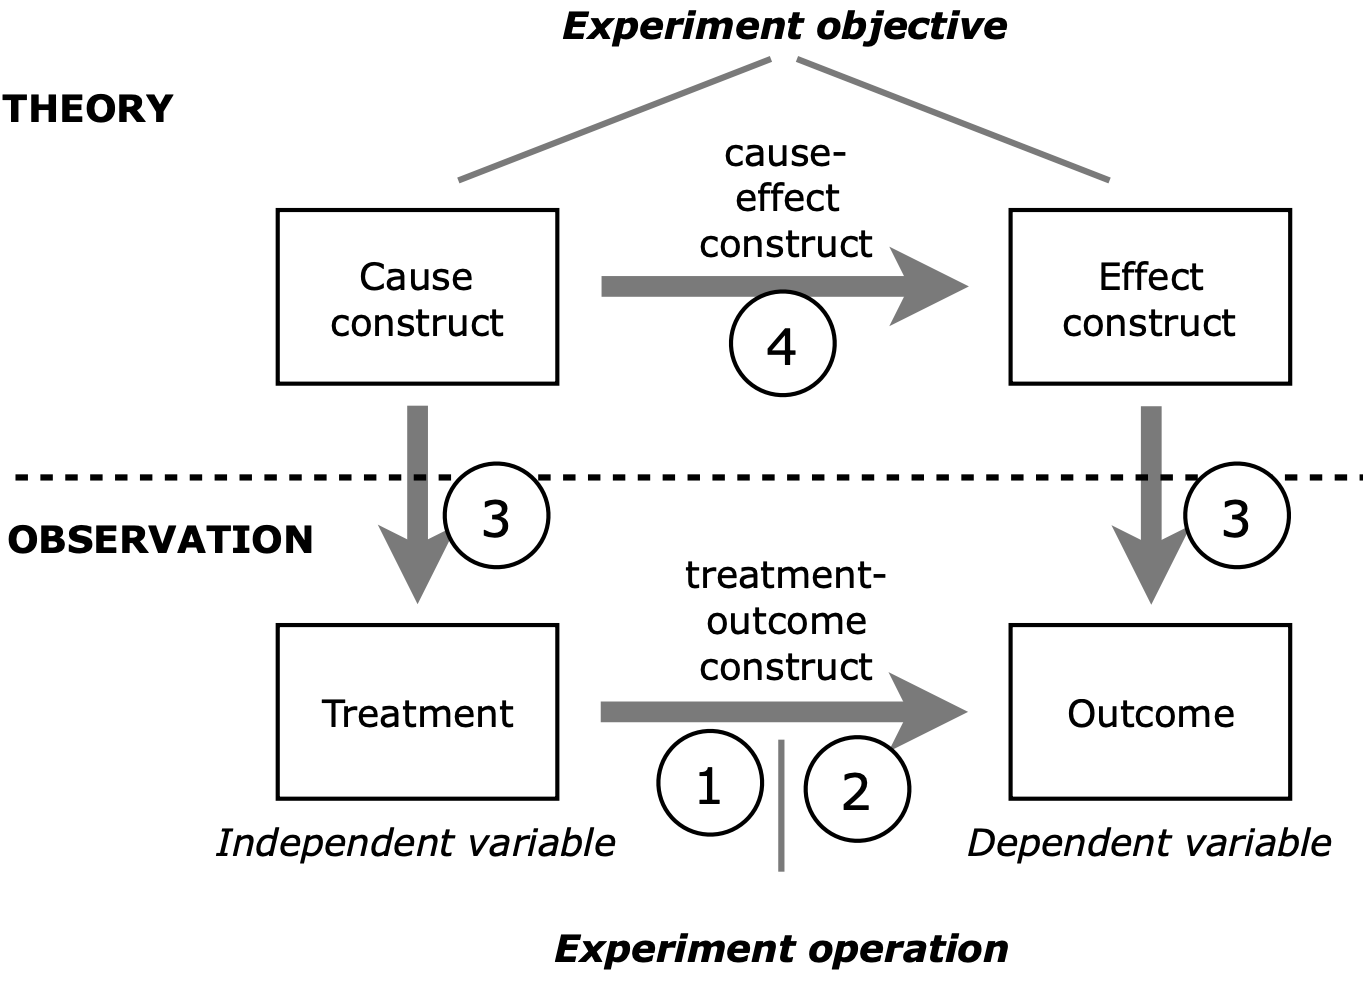
\includegraphics[width=0.75\textwidth]{images/threats-to-validity.png} 
	\caption{Experimental principles diagram showing threats. (1) Conclusion; (2) Internal; (3) Construct; and (4) External.}
	\label{fig:threats}
\end{figure}


\section{Conclusion validity}

Conclusion validity is the degree to which conclusions we reach about relationships in our data are reasonable.
\begin{itemize}
   \item  It affects the ability to draw correct conclusion about relations between treatment and outcome. \\
+ Choice of statistical tests \\
+ Choice of sample size \\
+ Measurement of the experiment
  \item Low Statistical Power \\
+ If power is low, there is a high risk that an erroneous conclusion is drawn.
\end{itemize}

\section{Internal validity}

Are there any other factors that may affect the results?
\begin{itemize}
  \item Were phenomena observed under special conditions \\
+ in the lab, close to a deadline, company risked bankruptcy, … \\
+ major turnover in team, contributors changed (open-source), …
  \item Similar observations repeated over time (learning effects)
  \item Correlation does not imply causation.
\end{itemize}

\section{Construct validity}

Do the operational measures reflect what the researcher had in mind?
\begin{itemize}
  \item Time recorded vs. time spent
  \item Execution time, memory consumption, … \\
+ noise of operating system, sampling method
  \item Human-assigned classifiers (bug severity, …) \\
+ risk for “default” values
  \item Participants in interviews have pressure to answer positively 
\end{itemize}

\section{External validity}

To what extent can the findings be generalized?
\begin{itemize}
  \item Does it apply to other languages? Other sizes? Other domains? Other systems?
  \item Background \& education of participants
  \item Simplicity \& scale of the team \\
+ small teams \& flexible roles vs. large organizations \& fixed roles
\end{itemize}

\newpage
% !TEX root = ../Victorvan Herel2025_Thesis.tex

\chapter{State-of-the-art: OSADL}\label{ch:related-work}

\comment{Victor: This chapter contains a lot of uncurated work, and the order or relevance of everything presented is not yet fixed in place. Here be dragons.}

The Open Source Automation Development Lab (OSADL) is a collaborative project that supports and promotes the use of open-source software, particularly Linux, in industrial and automation environments. OSADL focuses on ensuring that Linux and other open-source software components meet the stringent requirements of industrial applications, including real-time capabilities, legal compliance, and long-term maintenance.

Among the key activities of the OSADL organisation, \textbf{license compliance} is a dedicated subject it examines. OSADL helps member companies ensure their use of open-source software complies with licensing obligations by providing tools and services for legal audits and documentation that go deeper than those listed in Chapter~\ref{ch:background}~\cite{osadl-home}. \\

This aspect of the OSADL organisation is very interesting for this thesis, as it provides this dataset to the public for analysis and automated interaction. We will examine each of the relevant components.

\section{OSADL License Checklists}

The OSADL organization describes this project as follows: "Whenever Open Source software is copied and distributed which typically is permitted by every type of Open Source license, a number of obligations and prohibitions are imposed on the distributor. It is very common for the recipients of such software to recursively redistribute it in such a way that a chain of distributors and recipients is created – all of them having to fulfill the same license obligations. However, for the time being, there is no common understanding of how these obligations are to be fulfilled in detail which regularly leads to misunderstandings, conflicts and sometimes even to court cases.

This project is launched with the goal to generally establish checklists of obligations of commonly used Open Source software that are accepted by distributors and copyright holders and trusted by all members of the distribution chain."~\cite{osadl-license-checklists}

This description is executed by creating license checklists at the request of its members for specific licenses. These checklists provide an overview of all the obligations someone who wishes to use work licensed under it must fulfill, in a standardized way. For this, it uses several building blocks which we describe below. It should be noted that all raw data for each component is publicly available, and downloading this can be automated.

While it is possible that a checklist is formatted in a JSON format, and OSADL publishes a schema to validate against for these objects, we use the text format for explaining its workings in this thesis. \\

It is important to frame the checklists in the scope in which they are provided, quoted directly from the OSADL project page: "The checklists assume a situation where a licensee of Open Source software incorporates such software components into a product - either a physical device with installed software or a software distribution on a storage medium or on the Internet - and needs to establish appropriate processes in order to fulfill the imposed license obligations for legal compliance when conveying the product to customers."~\cite{osadl-license-checklists-scope}

This maps directly to the Full inclusion integration pattern we discussed in Chapter~\ref{ch:introduction}, limiting the use in particular to re-use of code and modification, as well as redistributing the completed result in some way.

\subsection{Checklist language}

Language used for checklists is fixed. It uses only defined terms, which sometimes allow freeform input (for example license names). These language constructs are separated into three main categories:

\begin{itemize}
	\item \textbf{Language elements:} Core elements of language that convey a particular meaning. These elements appear inspired by the language definitions used for RFC documents, as provided in RFC 2119. This inspiration however is not publicly cited on the web page. These elements include, but are not limited to, terms such as YOU MUST, YOU MUST NOT, USE CASE, ... . Notably, the OSADL authors have chosen to make these elements all uppercase to allow them to be distinguished easily.
	\item \textbf{Actions:} These elements are usually verbs, and are usually, but not always, what follows a language element in a provision. A couple of examples include terms such as: Publish, Provide, Add, Append, ... .
	\item \textbf{Terms:} These elements follow usually follow an action in provisions. This is the largest set of defined elements among these categories.
\end{itemize}

In effect, these allow us to write obligations in near-English sentences. For example, everyone understands "YOU MUST Provide License text" to mean just that, the requirement to provide the license's text if you use the covered work. How exactly these statements interact with each other is what we will cover next.

\subsection{Format description}

\subsubsection{Example: The MIT license}

To explain how the format works, we explain this by referring to an example checklist of the MIT license. That is provided verbatim in text form as follows.

\begin{verbatim}
	USE CASE Source code delivery OR Binary delivery
		YOU MUST Provide Copyright notices
		YOU MUST Provide License text
		YOU MUST Provide Warranty disclaimer
\end{verbatim}

We refer back to the MIT license text which was included in Chapter~\ref{ch:introduction}. Let's pick this checklist expression apart by listing all used definitions first, taking them verbatim from the dataset OSADL provides:

\begin{itemize}
	\item \textbf{USE CASE:} Sometimes the license obligations may allow the distributor to freely select between a number of optional use cases; the USE CASE language construct is introduced for this purpose. Several USE CASE language constructs to which the same license conditions apply may be combined using the OR language construct. If a particular USE CASE is mentioned repeatedly, e.g. once along with another USE CASE and once not, the obligations of all USE CASE sections must be fulfilled.
	\item \textbf{YOU MUST:} The YOU MUST language construct specifies an individual license obligation, i.e. what to do, probably among other things, to become license compliant. It may optionally be followed by indented language constructs such as ATTRIBUTE that further describe the license obligation.
	\item \textbf{OR:} When the OR language construct is used between elements of a condition, then the condition already applies, if only one element is fulfilled. When the OR language construct is used between obligations, then it is sufficient to fulfill at least one obligation. Note: The AND language construct is assumed by default between consecutive license obligations and attributes.
	\item \textbf{Provide:} The action to Provide means to make available particular material such as a license text to another natural or legal person. While the action to Forward is restricted to conveying existing material, the action to Provide expands the meaning in the sense that the material may be newly generated as long as it fulfills its purpose.
	\item \textbf{Source code delivery:} Licenses may treat the various aggregate states of deliverable software such as source, intermediate and object code differently. The term Source code delivery denotes a situation where source code is delivered, and no software component is included in the delivery without corresponding source code.
	\item \textbf{Binary delivery:} A software distribution may contain material not in a human-readable programming language, but in binary machine or intermediate code that was generated from the project's source code using a compiler. Some licenses may then impose disclosure obligations that may be fulfilled either by delivering the corresponding source code along with the binary code or by offering to do so at a later date. Irrespective of whether disclosure obligations exist and how they must be fulfilled, when software is delivered at least partly in object form then this is referred to as Binary delivery.
	\item \textbf{Copyright notice:} The Copyright notice indicates the name of the holder of the exclusive usage rights. In its minimal form, it may only contain a name in an obvious context. Usually, however, the name of the holder of the exclusive usage rights is preceded by the word 'Copyright', the © symbol or the letter c in parentheses '(c)', and a number or several numbers that indicate the year when the work was created." If the author is not the holder of the exclusive usage rights, the name of the holder of the exclusive usage rights may be followed by an attribution to the author.
	\item \textbf{License text:} The term License text denotes the unabbreviated original text of a particular license in its original language. It may either be printed on paper or contained in a data file on a medium using an obvious and well-known or an individually defined and specified character encoding.
	\item \textbf{Warranty disclaimer:} The license text may contain a clause or several clauses where the original authors refuse any warranty for malfunction or damages that may occur when using the licensed software. Such section is referred to as Warranty disclaimer.
\end{itemize}

With these definitions provided, we can pick apart the checklist line by line.

\begin{itemize}
	\item \verb*|USE CASE Source code delivery OR Binary delivery|: The subordinate elements of this checklist apply when distributing source code or binary forms of a project which is, in full or in part, subject to the terms of the license this checklist was made for.
	\item \verb*|YOU MUST Provide Copyright notices|: In these use cases, you are required to provide the copyright notice.
	\item \verb*|YOU MUST Provide License text|: You must also provide the unaltered license text.
	\item \verb*|YOU MUST Provide Warranty disclaimer|: And finally, you must provide the warranty disclaimer.
\end{itemize}

Thus, this checklist tells us exactly what we need to do when we want to redistribute work licensed under the MIT license in any code-bound form. Complying with all three requirements is as simple as including the full text of the original license, which includes the copyright notices (first line of the license) and the warranty disclaimer (last paragraph of the license in capitals).

This explanation aligns with our explanation in Chapter~\ref{ch:introduction} about how the MIT license works, and demonstrates how the format works. \\

\subsubsection{Formal definition}

The OSADL project also defines this format formally, where it is split in two sections. The first section of the format is displayed in the example, and contains these checklist items. We call this the primary section.

\comment{Victor: Fix this section. What is the goal?}


\subsection{Detecting license family based on a checklist}

OSADL also provides insight into how to determine the license family of a license. We recall from Chapter~\ref{ch:background} that this thesis considers each license to be part of one of two families: Permissive, or copyleft to any degree.

\comment{Victor: Fix this section as well.}

\begin{verbatim}
	USE CASE Source code delivery
		YOU MUST Provide License text
		YOU MUST NOT Modify Copyright notices
		IF Software modification
			YOU MUST Grant License
				ATTRIBUTE Original license
			YOU MUST Provide Copyright notices
		IF Commercial distribution
			YOU MUST Indemnify Other contributors
	USE CASE Binary delivery
		YOU MUST NOT Modify Copyright notices
		EITHER
			YOU MUST Provide Source code
		OR
			YOU MUST Provide Delayed source code delivery
				ATTRIBUTE Inform Recipient
			EITHER
				ATTRIBUTE Customary medium
			OR
				ATTRIBUTE Via Internet
				ATTRIBUTE Reasonable
		IF License change
			YOU MUST Use Identical License obligations
			YOU MUST Use Warranty disclaimer On behalf of Other contributors
				ATTRIBUTE Effective
			YOU MUST Use Liability disclaimer On behalf of Other contributors
				ATTRIBUTE Effective
			IF Service offerings
				ATTRIBUTE NOT Transferable
		IF Commercial distribution
			YOU MUST Indemnify Other contributors
\end{verbatim}

\subsection{Copyleft table}

OSADL also provides a JSON table that indicates for each license whether or not it has a copyleft clause. This value can be one of the following:

\begin{itemize}
	\item \textbf{Yes:} This indicates the license is part of the Copyleft Strict license family.
	\item \textbf{Yes (restricted):} This also logically implies the license is part of the Copyleft Limited license sub-family. Together with the licenses tagged Yes, this forms the full Copyleft license family.
	\item \textbf{No:} This maps to the permissive license family.
	\item \textbf{Questionable:} This final result implies that OSADL cannot come to a consensus on the presence of a copyleft clause in the license, thus implying that no general consensus exists. At the time of writing, this is assigned to the MS-PL and OpenSSL licenses in the dataset.
\end{itemize}

\subsection{Compatibility matrix}

OSADL also provides a curated matrix of compatibility between licenses, based on their checklists. This matrix is an aggregate product of the data elements and is therefore not new. The way these decisions are made however is not clearly documented.

Before we look into the specifics of this matrix, as it allows us to draw some valuable conclusions already, it is important to recall the scope in which the license checklists, which this matrix was based on, are constructed. This context was given earlier in this chapter.

Important definitions that result from combining two of these licenses in the scope of a compatibility question are the following:
\begin{itemize}
	\item \textbf{Leading license:} This is the license of the project that is the target of the inclusion. Code from the subordinate will end up in the project under this license.
	\item \textbf{Subordinate license:} This is the license that covers the code that is being taken.
\end{itemize}

To conclude, a compatibility result in the compatibility matrix provided by OSADL references a situation where one incorporates a part of the subordinate project into a leading project, and where the licenses of both projects are individual. This is still a case of the full inclusion pattern. \\

A compatibility result is either Yes, No, Unknown or Check Dependency. The first three are clear, but the Check dependency result needs to be clarified. OSADL introduces the concept of depending compatibility which defines that two licences are indeed incompatible, but allow a change to be made to the license configuration to make them compatible. This is to be read explicitly as: The configuration itself is \textbf{incompatible}, but one or both of the licenses allow themselves to be changed out for another license \textbf{explicitly} which does result in a compatible scenario.

\subsubsection{Expressing percentages}

In total, the dataset contains $116$ licenses, which results in $13456$ total combinations. However, we are only interested in $13340$ of these combinations, as $116$ of them are licenses being compared with themselves. These combinations are always compatible, and OSADL reports them as "Same." for this reason.

Looking further, we see that $1020$ of the combinations are listed as "Unknown". This leaves us with $12320$ assessed combinations of which:

\begin{itemize}
	\item $8812$ ($\sim 71.53\%$) are compatible.
	\item $3448$ ($\sim 27.99\%$) are not compatible.
	\item $60$ ($\sim 0.48\%$) fall in the case of depending compatibility.
\end{itemize}

An interesting finding arises when we combine this with the copyleft table, mapping "Yes" and "Yes (restricted)" to Copyleft, and "No" to Permissive. These results are shown below:

\begin{table}[h]
	\caption{OSADL compatibility in a copyleft-oriented view.}
	\label{tab:osadl-compat-numbers}
	\centering
	\begin{tabular}{l|ll}
		\hline
		\textbf{Subordinate \textbackslash Leading} & \textbf{Copyleft} & \textbf{Permissive} \\ \hline
		\textbf{Copyleft} & 812 total, 75 yes, 60 check dependency, 677 no & All 2465 no \\
		\textbf{Permissive} & 1729 total, 1498 yes, 231 no & All 7140 yes \\\hline
	\end{tabular}
\end{table}

This table shows a powerful property: If the leading license is permissive, we only need to know the license family of the subordinate license to be able to assess compatibility. \textbf{We conclude already that the license family is an important license property to automatically determine compatibility as part of the answer to RQ 1.}

Additionally, we see that a Copyleft/Copyleft combination is primarily incompatible, with some edge cases. These are always cases where the license lists licenses it is explicitly compatible with. For example, GPL-1.0-or-later is compatible with all future versions of the license by definition. (But not the other way around! Compatibility is a one-way relationship.)

Lastly, we observe that Copyleft/Permissive combinations are primarily compatible, but a not insignificant portion of combinations are incompatible. \\

To conclude this section, we can now make the powerful claim that if we know the license family a two licenses belong to, we can already answer $\sim 78.67\%$ of combinations, i.e. those where the leading license is permissive.

\section{Inducing the Permissive Leading effect logically}

In this last section, we present a logical argument as to why a permissive leading license allows for direct classification of combinations based on the license family the subordinate license belongs to. To do this, we consider the following definitions by OSADL: \comment{Victor: These need to be moved earlier. Also this needs to be argued about why these are disjoint.}
\begin{enumerate}
	\item \textbf{Compatibility is assumed, if:}
	\begin{itemize}
		\item compatibility with the other license is explicitly ruled in a particular license, or
		\item the two licenses in question both do not contain a copyleft clause, or
		\item the leading license contains a copyleft clause and the other license does not and also does nto impose any obligation that the first license does not allow to impose.
	\end{itemize}
	
	\item \textbf{Incompatibility is assumed, if:}
	\begin{itemize}
		\item incompatibility with another license is explicitly ruled in a particular license, or
		\item one license imposes an obligation that the other license does not allow to impose, or
		\item the two licenses in question both contain a copyleft clause and no license contains an explicit compatibility clause for this license combination.
	\end{itemize}
\end{enumerate}

These definitions already directly indicate why Permissive/Permissive is always compatible, namely it is defined as option 2 of OSADL's definition of compatibility. \\

This only leaves us to clarify why Permissive/Copyleft results in incompatible combinations at all times. To do this, we need to argue that these combinations always meet at least one of the three criteria for incompatibility.

To do this, we first recall what it means for a license to be in the copyleft license family: This means derivative works based on the covered work must be licensed equally in the strict case, or similarly in the limited case.
\begin{itemize}
	\item In the strict case, we land in bullet point two of incompatibility immediately. As we are trying to license the derivative work differently from the subordinate license.
	\item In the limited case, the same bullet point is reached as generally, the conditions under which the copyleft requirement may be waived do not include the full inclusion pattern. Alternatively, if the license is Copyleft Limited because it allows a specific subset of licenses to be used, we observe that these other licenses are also all in the Copyleft family, thus reverting to the base case in this bullet point.
\end{itemize}

As such, it is only logical that attempting to incorporate work licensed under a copyleft license using full inclusion in a work that is licensed under a permissive license creates an incompatible construction.

\chapter{New Ch3}

The Open Source Automation Development Lab (OSADL) is a collaborative project that supports and promotes the use of open-source software, particularly Linux, in industrial and automation environments. OSADL focuses on ensuring that Linux and other open-source software components meet the stringent requirements of industrial applications, including real-time capabilities, legal compliance, and long-term maintenance.

Among these key activities of the OSADL, \textbf{open source license compliance} is a key area it provides support in to its members. It does this in a number of ways that are of great interest for this thesis, with the goal of helping member companies and organizations in complying with obligations imposed by open source licensing and the way it interacts with their work. These tools it develops go a lot deeper than what the projects listed in Chapter~\ref{ch:background} aim to accomplish in certain areas~\cite{osadl-home}.

\section{Open source license checklists}

A first element we examine is the open source license checklists. At the time of writing, the OSADL provides what can be interpreted as a checklist of obligations to comply with when one wishes to interact with a specific license, for a set list of 116 licenses. This checklist has a relatively fixed format, which we will go over shortly before moving on to the next topic. \\

An open source license checklist is essentially formulated as a checklist with items to ensure software license compliance in general cases, using well-defined language elements. A checklist has two sections, an obligations section which describes the obligations imposed by a license and an optional supplements section which contains supplemental information which is sometimes already encoded in the obligations section.

It is important to understand that these checklists are still the result of manual curated work, as they are produced on the basis of requests made by members of the OSADL organization. Especially the supplements section, which often lists things like the presence of a copyleft clause, explicit (in)compatibilities, ... is the result of expert knowledge weighing in on the formulation. \\

The OSADL also makes clear in which context these license checklists are used. On this subject, it says the following: "The checklists assume a situation where a licensee of Open Source software incorporates such software components into a product - either a physical device with installed software or a software distribution on a storage medium or on the Internet - and needs to establish appropriate processes in order to fulfill the imposed license obligations for legal compliance when conveying the product to customers."~\cite{osadl-license-checklists-scope}

To draw a parallel to the integration types discussed in Chapter~\ref{ch:introduction}, this lines up fully with the full inclusion pattern, due to the sentence "... incorporates such software components into a product ...".

\subsection{Example: The MIT license}

To explain how the format works, we explain this by referring to an example checklist of the MIT license, shown below:

\begin{verbatim}
USE CASE Source code delivery OR Binary delivery
  YOU MUST Provide Copyright notices
  YOU MUST Provide License text
  YOU MUST Provide Warranty disclaimer
\end{verbatim}

The MIT license is an example of a license that does not need a supplements section, as it is very simple in scope and application, and does not list any specific interactions with other specific licenses. Still, we can learn some key facts from this about a license checklist's structure.

\begin{itemize}
	\item All obligations listed are "scoped" in one or more use cases, preceeded with the \texttt{USE CASE} statement. We will discuss the different use cases in a separate section.
	\item Obligations can be very specific in what they impose. In Chapter~\ref{ch:introduction}, we showed the text form of the license. Here we see that this license is split up into the copyright notice (the first line), the license text (lowercase paragraph) and the license disclaimer (uppercase paragraph). Each element is handled separately (though identically) in the license checklist.
\end{itemize}

It should also be noted that the OSADL does define each of the terms it uses (with some exceptions in the case of license names, ...). For example, the following definitions exist quoted directly from the OSADL data:

\begin{itemize}
	\item \textbf{USE CASE:} Sometimes the license obligations may allow the distributor to freely select between a number of optional use cases; the USE CASE language construct is introduced for this purpose. Several USE CASE language constructs to which the same license conditions apply may be combined using the OR language construct. If a particular USE CASE is mentioned repeatedly, e.g. once along with another USE CASE and once not, the obligations of all USE CASE sections must be fulfilled.
	\item \textbf{YOU MUST:} The YOU MUST language construct specifies an individual license obligation, i.e. what to do, probably among other things, to become license compliant. It may optionally be followed by indented language constructs such as ATTRIBUTE that further describe the license obligation.
	\item \textbf{Provide:} The action to Provide means to make available particular material such as a license text to another natural or legal person. While the action to Forward is restricted to conveying existing material, the action to Provide expands the meaning in the sense that the material may be newly generated as long as it fulfills its purpose.
	\item \textbf{Source code delivery:} Licenses may treat the various aggregate states of deliverable software such as source, intermediate and object code differently. The term Source code delivery denotes a situation where source code is delivered, and no software component is included in the delivery without corresponding source code.
	\item \textbf{Binary delivery:} A software distribution may contain material not in a human-readable programming language, but in binary machine or intermediate code that was generated from the project's source code using a compiler. Some licenses may then impose disclosure obligations that may be fulfilled either by delivering the corresponding source code along with the binary code or by offering to do so at a later date. Irrespective of whether disclosure obligations exist and how they must be fulfilled, when software is delivered at least partly in object form then this is referred to as Binary delivery.
	\item \textbf{Copyright notice:} The Copyright notice indicates the name of the holder of the exclusive usage rights. In its minimal form, it may only contain a name in an obvious context. Usually, however, the name of the holder of the exclusive usage rights is preceded by the word 'Copyright', the © symbol or the letter c in parentheses '(c)', and a number or several numbers that indicate the year when the work was created." If the author is not the holder of the exclusive usage rights, the name of the holder of the exclusive usage rights may be followed by an attribution to the author.
	\item \textbf{License text:} The term License text denotes the unabbreviated original text of a particular license in its original language. It may either be printed on paper or contained in a data file on a medium using an obvious and well-known or an individually defined and specified character encoding.
	\item \textbf{Warranty disclaimer:} The license text may contain a clause or several clauses where the original authors refuse any warranty for malfunction or damages that may occur when using the licensed software. Such section is referred to as Warranty disclaimer.
\end{itemize}

In these definitions, we see the three separated elements from the MIT license returning as defined constructs which are defined generally, and thus also applicable to other license models.

\subsection{Detecting copyleft clauses based on a license checklist}\label{sec:detect-copyleft-from-license-checklist}

An interesting property of these license checklists is that, while always explicitly mentioned in the supplements section, a copyleft property can also be inferred through the obligations section. We show this property with an example, namely the GPL-1.0-only license.

\comment{Victor: See if there's a better way to lay this out.}

\begin{verbatim}
USE CASE Source code delivery
    YOU MUST Provide Copyright notices
        ATTRIBUTE Highlighted
        ATTRIBUTE Appropriately
    YOU MUST Provide Warranty disclaimer (Warranty disclaimer)
        ATTRIBUTE Highlighted
        ATTRIBUTE Appropriately
    YOU MUST NOT Modify License notices
    YOU MUST NOT Modify Warranty disclaimer (Warranty disclaimer)
    YOU MUST Provide License text
    IF Software modification
        YOU MUST Grant License
            ATTRIBUTE Original license
        YOU MUST Provide Modification notice
        YOU MUST Provide Modification date
        IF Interactive
            YOU MUST Display License announcement
            YOU MUST Display Copyright notices
            YOU MUST Display Warranty disclaimer
            YOU MUST Reference License text
    YOU MUST NOT Restrict Granted rights
USE CASE Binary delivery
    YOU MUST Provide Copyright notices
        ATTRIBUTE Highlighted
        ATTRIBUTE Appropriately
    YOU MUST Provide Warranty disclaimer (Warranty disclaimer)
        ATTRIBUTE Highlighted
        ATTRIBUTE Appropriately
    YOU MUST NOT Modify License notices
    YOU MUST NOT Modify Warranty disclaimer (Warranty disclaimer)
    YOU MUST Provide License text
    EITHER
        YOU MUST Provide Source code
            ATTRIBUTE Machine-readable
    OR
        YOU MUST Provide Written offer (Written offer)
            ATTRIBUTE Duration 3 years
            ATTRIBUTE To Any third party
            ATTRIBUTE No profit
            ATTRIBUTE Delayed source code delivery
                ATTRIBUTE Machine-readable
    IF Software modification
        YOU MUST Grant License
            ATTRIBUTE Original license
        YOU MUST Provide Modification notice
        YOU MUST Provide Modification date
        IF Interactive
            YOU MUST Display License announcement
            YOU MUST Display Copyright notices
            YOU MUST Display Warranty disclaimer
            YOU MUST Reference License text
    YOU MUST NOT Restrict Granted rights
(... 73 license compatibility/incompatibility statements ...)
COPYLEFT CLAUSE Yes
\end{verbatim}

In this example, the supplement (represented by the last two lines) mentions correctly that a copyleft clause is indeed present. However, we see this requirement returning in the obligations section, namely in the following lines:

\begin{verbatim}
USE CASE Source code delivery
    ...
    IF Software modification
        YOU MUST Grant License
            ATTRIBUTE Original license
    ...
USE CASE Binary delivery
    EITHER
        YOU MUST Provide Source code
            ATTRIBUTE Machine-readable
    OR
        YOU MUST Provide Written offer (Written offer)
            ATTRIBUTE Duration 3 years
            ATTRIBUTE To Any third party
            ATTRIBUTE No profit
            ATTRIBUTE Delayed source code delivery
                ATTRIBUTE Machine-readable
    IF Software modification
        YOU MUST Grant License
            ATTRIBUTE Original license
        ...
\end{verbatim}

When summarized like this, we see a strict copyleft requirement emerging. Namely, in both delivery use cases, you are required to grant your changes under the original license (\textbf{but not the original copyright notices}). Even more so, in Binary delivery, you are also obligated to provide source code, either immediately or in the form of a written offer valid for 3 years. This last obligation forces you into the Source code delivery use case in both cases, where the copyleft requirement for the source code also holds.

Logically, to comply with the obligations in this checklist which represent the license itself, regardless of what you do, you must provide your derivative work in source code form and optionally binary form under the same license. (But again, not the original copyright notices.)

\section{Notable use cases}

Before we continue with other ground truth data sources the OSADL provides, we take a moment to consider the other noteworthy use cases the OSADL defines and uses in their license checklists. For clarity, these are the "arguments" to a USE CASE statement in the checklist.

First, we recall that we already identified what "Source code delivery" and "Binary delivery" means. With this in mind, the following terms of interest remain:

\begin{itemize}
	\item \textbf{X delivery Of Combined library:} The OSADL defines a Combined library as follows: "If two or more libraries are copied into a single library that offers the functionality of the library components all together, but without applying any modifications to them, then the resulting library is referred to as a Combined library."
	
	As a result, delivery (both binary and source code) of such a work fall under this work, and are used in the LGPL-family of licenses. This family is a non-strict copyleft license, and as such mentions libraries explicitly.
	
	\item \textbf{X delivery of Combined work:} Likewise, the OSADL provides the following definition for the term Combined work: "A Combined work is created when a work consists of two or more originally separated components that are combined in such a way that they form a new work no longer allowing them to operate independently."
	
	This has a similar implication, but is more general on one hand, not limiting itself to libraries, but also more specific in the sense that the work must not be able to be separated as a result. Regrettably, which functions are used as a benchmark to determine this treshold of functionality is left rather vague. We see this use case also used by the LGPL family of licenses.
	
	\item \textbf{Combined work delivery:} The Sleepycat license is the only license to use this use case, and it does so to enforce the copyleft property on what the OSADL defines as a Combined work (see the bullet point above). In this use case, one is required to either include the source code in the combined work, or to provide delayed source code delivery of combined work for no profit, similarly to the GPL-1.0-only example previously handled. Note however that this license does not define a time window in which this delayed delivery must be performed. We will return to the Sleepycat license later, as it appears to be a difficult license to work with in particular.
	
	\item \textbf{Binary delivery of Linked work:} The OSADL defines a Linked work as: "A work may be linked to another work at compile time or at run time in which case the other work is referred to as Linked work."
	
	Examples of this arise in any programming language when one uses a library in their code without including the library itself as a baked-in option. (For example, \texttt{requirements.txt} for Python, module imports for Go, classpath linking for Java using Maven or Gradle, or any other pattern in which the dependencies of a project are described in a declarative way, based on which automated tooling can independently retrieve the library files needed itself.) The \textbf{library} is the linked work.
	
	This has a variant, namely \textbf{Binary delivery of Linked work With Header files OF Library Included In Linked work}. \comment{Victor: What in the world does this mean? The linked work IS the library. It includes its own header files?}
	
	Once again, the LGPL family uses these terms explicitly. It is also used by the Artistic-2.0 license.
	
	\item \textbf{Font, Image, Work, ... delivery:} The delivery word can be used with a number of various other terms, indicating that the license in question covers this "type" of work separately.
	
	These terms are used by more general licenses that don't specifically cover code, like the CC family of licenses. However, we also see these elements appearing in the Bitstream-Vera and the OFL-1.1 license.
	
	As the term "Work" is very general, we call out its OSADL definition explicitly to clarify it: "Copyright law specifies a Work as any artifact that was created by a human being, can be perceived by a human being and possesses individual characteristics that are attributable to a human being. In the context of software licensing, the term Work is used to denote a collection of software components that are conveyed as a whole under the same license or, if compatible, under the same group of applicable licenses."
	
	\item \textbf{Network service:} This does not constitute delivery in the traditional sense, rather, the OSADL defines it as follows: "The term Network service is used to describe a situation when a provider does not convey a software application in binary form to a customer, but installs it on a network-capable computer and let customers use the application by communicating with it via a network link."
	
	This use case is outlined explicitly by the AGPL family of licenses, which is known for specifically differing from the GPL family of licenses because it covers the "network service loophole". This use case is also explicitly covered by the AFL-3.0 and the OFL-3.0. It should be noted that this use case is generally understood not to be covered by any variation of the term "Derivative work" in copyright law, as one is using the work themselves and in doing so, is providing a different service to the end users.
\end{itemize}

\section{Copyleft table}

Aside from the now examined license compliance checklists, the OSADL makes available a distilled source of information. Namely, a table that lists the copyleft status of each of the licenses in the raw data. It should be noted that while the licenses themselves list the copyleft property in their license checklist supplements, this table is actually more specific.

This is because this table goes deeper than a yes/no answer. Namely, it lists the following possibilities:

\begin{itemize}
	\item \textbf{No:} Licenses with this classification are permissive.
	\item \textbf{Yes:} Licenses with this classification are Strict Copyleft family.
	\item \textbf{Yes (restricted):} Licenses with this classification are in the Copyleft Limited family.
	\item \textbf{Questionable:} This classification is used for two licenses, namely the MS-PL and OpenSSL licenses. We examine the license checklist of each of these separately, using the process outlined in Heading~\ref{sec:detect-copyleft-from-license-checklist} to classify these licenses ourselves.
	
	\comment{Victor: Fill this in.}
\end{itemize}

\section{Compatibility matrix}

Based on these license checklists, we can consider a situation in which two license checklists are checked against eachother, one in a leading position and the other in a subordinate context. This context is derived from the context of an individual license checklist. Recall, that a license checklist itself is made in the context of the licensed work being included in another work, without specifying what the other work is licensed under.

In this section, we examine the situation that occurs when we do know what the including work is licensed as. In this sense, we define the leading license as the license that governs the including work. The work that is being included, in part or in full, is governed under the subordinate license. \\

This construction is a construction that the OSADL has already examined for a lot of the licenses it covers. It provides the raw data of these experiments, which are still the result of human curation, as a matrix which we can examine. In this matrix, we have the following types of results:

\begin{itemize}
	\item \textbf{Yes:} This result indicates that the obligations imposed by both licenses do not conflict. However, the combined work still must abide by both licenses' obligations. As such, this compatibility is only theoretical, not practical.
	\item \textbf{No:} This result indicates incompatibility. This means there is some obligation combination that causes problems when applied.
	
	As we will see, the copyleft property of a license is an important thing to know here. For instance, if the leading license is permissive, and the subordinate license is copyleft in any way, then by definition the combination cannot be compatible. This is because the combination would become a derivative work of the copyleft licensed work, thus requiring it as a whole to be similarly licensed.
	\item \textbf{Check dependency:} A third option is what the OSADL defines as Depending compatibility. This is a combination of two licenses in the context previously discussed, which in the definition of the two participating licenses is incompatible. However, either one of the licenses allows it to be replaced at any time with another license it specifies, usually a newer version of the same license, which does make the combination compatible. These cases are rare, and are flagged separately. As an example, an LGPL license can generally be upgraded into its GPL variant, dropping the special provisions surrounding linking. LGPL licenses are not compatible with GPL licenses, but naturally GPL licenses are compatible with themselves.
	
	\item \textbf{Unknown:} Not all license combinations were evaluated by the OSADL. In this case, the field is listed as this value.
\end{itemize}

\subsection{Identifying clusters of interest}

Given the ground truth information in this compatibility matrix, it is useful to examine which information we need to correctly classify most of license combinations within it. This will in turn allow us to perform automated querying for licenses in a smart way, without having to resort to the infeasible per-combination query behavior. By means of a spreadsheet which we add specific columns to, we can attempt to identify useful classes of interest.

If we make this spreadsheet with one row for each combination, and add two columns indicating the OSADL-provided copyleft license table entry for the leading and the subordinate license, we can already make some important distinctions:

\begin{enumerate}
	\item \textbf{Permissive-X} (9775 / 13340)\textbf{:} When the leading license is permissive (= No in the copyleft table), it is immediately obvious that we can produce an accurate decision if we know the copyleft state of the subordinate license. Namely, if it is permissive, the combination is always compatible. If it is any form of copyleft, it is always incompatible. If the subordinate license is classed as Questionable, the result is unfortunately always unknown. Aside from this, this class does not have any Unknown classifications.
	
	In numbers, we see this class containing the following results:
	
	\begin{table}[h]
		\caption{Table for Permissive-X compatibility class}
		\label{tab:permissive-x-table}
		\centering
		\begin{tabular}{|cc|cc|c|}
			\hline
			\multicolumn{2}{|c|}{\textbf{Permissive-Permissive}} & \multicolumn{2}{|c|}{\textbf{Permissive-CopyleftAny}} & \textbf{Permissive-Questionable} \\
			Yes & Unknown & No & Unknown & Unknown \\
			7140 & 0 & 2465 & 0 & 170 \\\hline
			\multicolumn{5}{|c|}{9775 total combinations (out of 13340 $\sim$ 73.276\%)} \\
			\hline
		\end{tabular}
	\end{table}
	
	\item \textbf{CopyleftAny-Permissive} (2465 / 13340)\textbf{:} When the leading license is copyleft, and the subordinate license is permissive, generally, we expect the combination to be compatible unless there is some specific cause for it not to be. This is because permissive licenses are generally permissive in how the work covered under them are used, and thus any conflicts should arise from the copyleft leading license disallowing something that the permissive license still requires in terms of material reproduction. This is supported by the number of records in each category, provided as follows:
	
	\begin{table}[h]
		\caption{Table for Copyleft-Permissive compatibility class}
		\label{tab:copyleft-permissive-table}
		\centering
		\begin{tabular}{|c|c|c|}
			\hline
			\multicolumn{3}{|c|}{\textbf{CopyleftAny-Permissive}} \\
			Yes & No & Unknown \\
			1498 ($\sim$ 60.993\%) & 231 ($\sim$ 9.493\%) & 736 ($\sim$ 29.858\%) \\\hline
			\multicolumn{3}{|c|}{2465 total combinations (out of 13340 $\sim$ 18.2478\%)} \\
			\hline
		\end{tabular}
	\end{table}
	
	\item \textbf{CopyleftAny-CopyleftAny} (812 / 13340)\textbf{:} Y/N/CheckDep
	
	\item \textbf{CopyleftAny-Questionable} (58 / 13340)\textbf{:} Unknown/N
\end{enumerate}

\newpage
% !TEX root = ../Victorvan Herel2025_Thesis.tex

\chapter{Conclusion}\label{ch:conclusion}

The first paragraph of the conclusion is usually a short review of this paper/thesis goals, problems, and context. 

After that we generally cover the following main points in the next paragraphs:

\begin{itemize}
\item \textbf{Summary of Results.} 
   In a paper/thesis, we probably have many pages in previous sections presenting results. 
   Now in the conclusion, it is time to put the most important results here for the reader. 
   Especially research with measurable results, we highlight the numbers here. 
\item \textbf{Main Findings / Conclusions.} 
   Many times, we have a result but based on its number we can draw a conclusion or formulate a finding on top of it. 
   Even if it was previous discussed in an earlier section, we need to re-state here. 
\item \textbf{Contributions.} 
   If we presented/discussed the main contributions of this research in the introduction, then we need to do again in the conclusion.
   Do not repeat verbatim what was written in previous sections. 
   In the conclusion, we expect contributions to be more detailed and linked to the results/findings when possible.
\end{itemize}

Avoid generic conclusion sentences that could be applied to anything. 
For example, "Our technique showed good results which were beneficial to answer our research questions. 
Our work can be used by other researchers to better understand our domain."
Instead, go for more specific detailed results.
For example, "Our technique showed a precision of 75\% which was 15\% higher than the baseline comparison. 
Based on this we can see that ..."

The final paragraph (or paragraphs) of the conclusion is about future research. 
We can create a separate subsection for it if there are multiple paragraphs dedicated to future work. 
Just be aware, it is not a good sign if future research content is longer than what we wrote for the previous paragraphs in the conclusion.


\newpage
\bibliographystyle{unsrt}
\bibliography{references}
\addcontentsline{toc}{section}{References}

\end{document}